\documentclass[11pt]{article}
\usepackage[utf8]{inputenc} % Required for inputting international characters
\usepackage[T1]{fontenc} % Output font encoding for international characters
%TODO Decide between Palantino and Computer modern
\usepackage{mathpazo} % Palatino font
\usepackage{subfiles}
\usepackage{multirow}
\usepackage{amssymb}
\usepackage{amsmath}
\usepackage[margin=1in]{geometry}
\usepackage{enumitem}
\usepackage{caption}
\usepackage{graphicx} %package to manage images
\setlength{\emergencystretch}{10pt} % handles text going outside of boxes
\setcounter{tocdepth}{2} %makes the table of contents only go 2 layers deep
\usepackage[export]{adjustbox} % for frames on figures
\usepackage{multicol}
%TODO Decide if we want first paragraph tabbed after section
%\usepackage{indentfirst}
\begin{document}
%----------------------------------------------------------------------------------------
%	TITLE PAGE
%----------------------------------------------------------------------------------------
\begin{titlepage} % Suppresses displaying the page number on the title page and the subsequent page counts as page 1
	\newcommand{\HRule}{\rule{\linewidth}{0.5mm}} % Defines a new command for horizontal lines, change thickness here
	
	\center % Centre everything on the page
	
	%------------------------------------------------
	%	Headings
	%------------------------------------------------
	
	\textsc{\LARGE McGill University}\\[1.5cm] % Main heading such as the name of your university/college

	\textsc{\large COMP 551 - Applied Machine Learning}\\[0.5cm] % Minor heading such as course title
	
	%------------------------------------------------
	%	Title
	%------------------------------------------------
	
	\HRule\\[0.4cm]
	
	{\huge\bfseries Assignment 2 Report}\\[0.4cm] % Title of your document
	
	\HRule\\[1.5cm]
	
	%------------------------------------------------
	%	Author(s)
	%------------------------------------------------
	
	\begin{minipage}{0.5\textwidth}
		\begin{flushleft}
			\large
			Written by:\\
			Asher \textsc{Wright} - {\small 260559393}
		\end{flushleft}
	\end{minipage}
	~
	\begin{minipage}{0.4\textwidth}
		\begin{flushright}
			\large
			Due to:\\
			Prof.  \textsc{Chandar} 
		\end{flushright}
	\end{minipage}
	

	
	%------------------------------------------------
	%	Date
	%------------------------------------------------
	
	\vfill\vfill\vfill % Position the date 3/4 down the remaining page
	
	{\large February 12, 2018} 
		%----------------------------------------------------------------------------------------
	
	\vfill % Push the date up 1/4 of the remaining page
\end{titlepage}

\pagebreak

\section*{Linear Classification and Nearest Neighbour Classification}
\subsection*{1. Dataset 1}
The first dataset, DS1, was created as indicated in the handout. Please note that I decided to split up the data into different text files. I first split it into testing and training (as was given in assignment 1), and then I further split it up into positive and negative classes. Another, more scalable, option would be to add a column to the data called "label", but with two classes I found this method easier.

\subsection*{2. LDA with Dataset 1}
Below are the computed performance measures for dataset 1 with LDA classification.\\
\begin{tabular}{llllll}
Best fit accuracy & 95.08 \% &  &  &  &  \\
Precision         & 95.77 \% &  &  &  &  \\
Recall            & 94.33 \% &  &  &  &  \\
F-measure         & 95.05 \% &  &  &  &  \\
                  &          &  &  &  &  \\
\end{tabular}
\\
\noindent
The coefficients learnt were the following:\\
$w$ = [-14.70625916, 8.72333061, 6.06823166, 3.39412552, 10.23338177, 4.19114737, -17.87277904, 24.77351351, 30.34024193, -9.18815402, 13.27738285, 12.89340784, -16.32857775, -13.64881951, 5.89264418, -13.54701867, -30.67490656, 6.98491646, 0.99426985, 5.20896759]\\
$w_0$ = -28.0514877938
\subsection*{3. k-NN with Dataset 1}
Figure 1 shows how the $F_1$ measure changed as k was increased from 1 to 150. I only chose odd numbers of k to prevent having to deal with ties. As it would be messy to list the performance for every 75 k value, I instead list the performances every 10, as well as the best. The performances for each value of k are given below in Table 1. 

\begin{figure}[h]
\centering
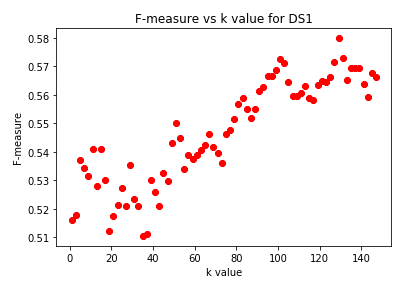
\includegraphics[width=0.5\textwidth]{ds1_f_k}
\caption{F-measure vs k value for NN, dataset 1}
\end{figure}

\begin{figure}[h]
\centering
\caption*{Table 1: F-measure values}
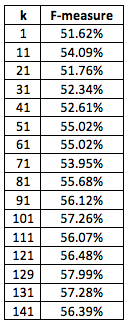
\includegraphics[width=0.2\textwidth]{ds1_f_k_values}
\end{figure}

This classifier does much worse than LDA. The linear approach yields around a 95\% $F_1$ measure, whereas this reaches about 58\% at the maximum, at a k value of 129. Generally, the k-NN classifier improves as k increases, up to about 100, where it then fluctuates. Depending on the (randomly) generated data, the optimal value of k could change greatly. It would be a good idea to use a separate set of data to properly select a value of k.\\

\noindent
Below are the computed performance measures for dataset 1 with k-NN (k = 129) classification.\\
\begin{tabular}{llllll}
Best fit accuracy & 56.42 \% &  &  &  &  \\
Precision         & 55.97 \% &  &  &  &  \\
Recall            & 60.17 \% &  &  &  &  \\
F-measure         & 57.99 \% &  &  &  &  \\
                  &          &  &  &  &  \\
\end{tabular}
\\

\subsection*{4. Dataset 2}
Again, as for dataset 1, I decided to save multiple text files, split into the testing and training sets, as well as the positive and negatively classified sets. I did this instead of using a label column.

\subsection*{5. LDA \& k-NN with Dataset 2}
Below are the computed performance measures for dataset 2 with LDA classification.\\
\begin{tabular}{llllll}
Best fit accuracy & 55.83 \% &  &  &  &  \\
Precision         & 55.52 \% &  &  &  &  \\
Recall            & 58.67 \% &  &  &  &  \\
F-measure         & 57.05 \% &  &  &  &  \\
                  &          &  &  &  &  \\
\end{tabular}\\

Next, k-NN was performed with k varying again. The values for k this time can be seen in Figure 2, below. It is worth noting that there is no clear trend at all with how k changes and the $F_1$ measure for k-NN with dataset 2.
\begin{figure}[h]
\centering
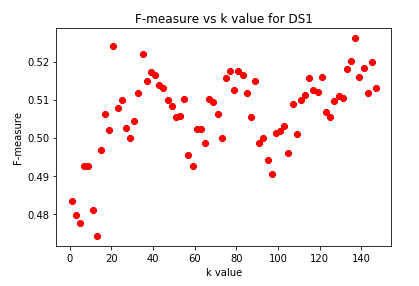
\includegraphics[width=0.5\textwidth]{ds2_f_k}
\caption{F-measure vs k value for NN, dataset 2}
\end{figure}

The k corresponding to the highest f value was k = 137, which yielded an F-measure of 52.61\%. Using this value, the following performance measures were found for dataset 2 with k-NN classification.

\begin{tabular}{llllll}
Best fit accuracy & 56.17 \% &  &  &  &  \\
Precision         & 57.25 \% &  &  &  &  \\
Recall            & 48.67 \% &  &  &  &  \\
F-measure         & 52.61 \% &  &  &  &  \\
                  &          &  &  &  &  \\
\end{tabular}\\
Now both of the classification methods do not perform well. With many different blobs of data, neither method is able to classify well. LDA still performs better than k-NN, which is against what I would have guessed. Since there are different clumps of data, with certain covariances around certain means, I would have guessed that nearest neighbours would have been able to be quite accurate within those clumps, but this appears to not be the case. 


\subsection*{6. Final comments}
With the first dataset, which was created using a single gaussian, LDA classification was very effective. K-NN was not effective in this case. With the second dataset, both classifiers had about the same accuracy, which was very poor (~56\%). As well, the precision of each classifier was about the same. However, one thing that is interesting is that the recall of the k-NN classifier was much lower than that of LDA, and thus LDA had a higher F-measure.


\end{document}